\documentclass{beamer}

\usepackage{amsmath,amssymb,amsfonts,dcolumn,color,graphicx,graphics,setspace,latexsym,setspace,lscape,subfigure,placeins,epsfig,hyperref}
\usepackage{eulervm}
\usepackage[utf8]{inputenc}
\usepackage{csquotes}

\usepackage{tikz}
\usetikzlibrary{trees,shapes}
\usetheme{Kalgan}


\setbeamercovered{highly dynamic}
\setbeamersize{text margin left=10pt}

\newcommand{\be}{\begin{equation}}
\newcommand{\ee}{\end{equation}}
\newcommand{\lb}{\left}
\newcommand{\rb}{\right}



\begin{document}

\title{Linux WTF?}
\subtitle{Eine Einführung in das Betriebssystem Linux}
\author{Benedikt Schmitz}
%\institute[FUG]{FiwiAn UG}
\date{}



	\begin{frame}[plain]
	  \titlepage
	\end{frame}
	\begin{frame}
  		\frametitle{Outline}
		\tableofcontents
	\end{frame}
%%%%%%%%%%%%%%%%%%%%%%%%%%%%%
%%%% Inhalte 
%%%%%%%%%%%%%%%%%%%%%%%%%%%%%
	\section{Linux -- kann man das Essen?}
	    \subsection{Installation}
	        \begin{frame}
          		\frametitle{Linux -- kann man das Essen?}
            		\begin{center}
                		\begin{minipage}{0.44\textwidth}
                		    \begin{itemize}
                		        \item Installation
                		        \item Vor und Nachteile
                		    \end{itemize}
                		\end{minipage}%
            		\end{center}
        	\end{frame}
        	
	        \begin{frame}
          		\frametitle{Installation via USB}
          		%-- welche Einstellungen bei der Installation? Swap, zweite platte für /home
        		\begin{minipage}{0.60\textwidth}
        		    \begin{itemize}
        		        \item SWAP $\to$ für den Notfall mit hoher RAM Auslastung $\sim$ so groß wie RAM
        		        \item /home kann mit neuer Partition angelegt werden.
        		        \item Installer übernimmt Großteil :)
        		        \item Einstecken und Anweisungen folgen...  
        		    \end{itemize}
        		\end{minipage}%
        		\begin{minipage}{0.39\textwidth}
        		    \includegraphics[scale=0.3]{bilder/20120220.png}\footnote{http://smbc-comics.com/comic/2012-02-20}
        		\end{minipage}
        	\end{frame}
        	
	    \subsection{Vorteil von Linux?}
	        \begin{frame}
          		\frametitle{Vor- und Nachteile von Linux}
        		\begin{minipage}{0.8\textwidth}
        		    \begin{itemize}
        		        \item[+] Open Source
        		        \item[+] Kein Anti-Virus nötig
        		        \item[+] Viele Alternativen (Texteditor, Distros, ...)
        		        \item[+] Kommandozeile
        		        \item[+] Kein Reboot nötig
        		        \item[+] Niedrige Ressourcenanforderungen
        		        \item[+] Multitasking
        		        \item[+] Wenig Speicherbedarf
        		        \item[+] Viele Dateiformate
        		        \item[--] Treiber
        		        \item[--] Lernkurve
        		        \item[--] Software Alternativen (Photoshop, Microsoft Office,  Adobe, ...)
        		        \item[--] Games
        		    \end{itemize}
        		\end{minipage}%
        	\end{frame}
        	
    \section{Linux $\leftrightarrow$ Windows: Unterschiede...}
        \begin{frame}
      		\frametitle{Linux $\leftrightarrow$ Windows: Unterschiede...}
        		\begin{center}
            		\begin{minipage}{0.44\textwidth}
            		    \begin{itemize}
            		        \item ... Konzeptionell
            		        \item ... Ordnerbaum
            		        \item ... Nutzer
            		        \item ... Installation von Software
            		    \end{itemize}
            		\end{minipage}%
        		\end{center}
    	\end{frame}
        \subsection{... Konzeptionell}
            \begin{frame}
          		\frametitle{Kernel/Hardware/User space}
                \begin{center}
            		\begin{minipage}{0.54\textwidth}
            		    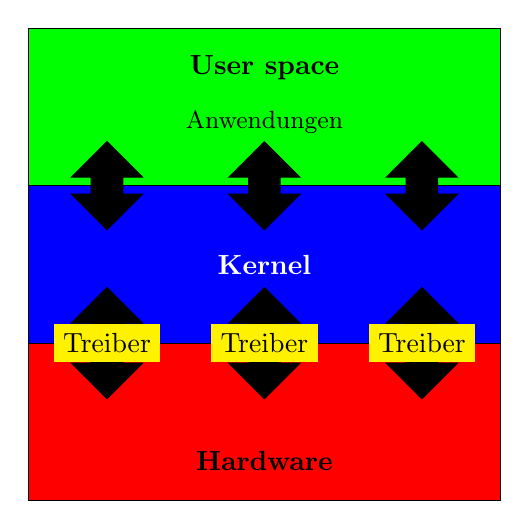
\begin{tikzpicture}
            		        \draw[fill=green] (-3,3) rectangle (3,1);
            		        \draw[fill=blue] (-3,1) rectangle (3,-1);
            		        \draw[fill=red] (-3,-1) rectangle (3,-3);
            		        % Enter label
            		        \node at (0,2.5) {\textcolor{black}{\textbf{User space}}};
            		        \node at (0,1.8) {\textcolor{black}{\small{Anwendungen}}};
            		        \node at (0,0) {\textcolor{white}{\textbf{Kernel}}};
            		        \node at (0,-2.5) {\textcolor{black}{\textbf{Hardware}}};
            		        % Pfeile
            		        \node[draw,fill, shape=double arrow,rotate=90] at (-2,+1) {-- --}; 
            		        \node[draw,fill, shape=double arrow,rotate=90] at (0,+1) {-- --};
            		        \node[draw,fill, shape=double arrow,rotate=90] at (+2,+1) {-- --};
            		        
            		        \node[draw,fill, shape=double arrow,rotate=90] at (-2,-1) {-- -- --}; 
            		        \node[draw,fill, shape=double arrow,rotate=90] at (0,-1) {-- -- --};
            		        \node[draw,fill, shape=double arrow,rotate=90] at (+2,-1) {-- -- --};
            		        %Treiber:
            		        \node[rectangle, fill=yellow] at(-2,-1) {\textcolor{black}{Treiber}};
            		        \node[rectangle, fill=yellow] at(0,-1) {\textcolor{black}{Treiber}};
            		        \node[rectangle, fill=yellow] at(2,-1) {\textcolor{black}{Treiber}};
            		    \end{tikzpicture}
            		\end{minipage}
        		\end{center}
        	\end{frame}
        	
        \subsection{... Ordnerbaum}
            \begin{frame}
          		\frametitle{Ordnerhierarchie/backups}
        		\begin{center}
        		    \begin{tikzpicture}
        		        \node{/ }[edge from parent fork down]
                        child{node[rectangle,draw=white]{bin}}
                        child{node[rectangle,draw=white]{etc}}
                        child{node[rectangle,draw=white]{home}
                            child{node[rectangle,draw=white]{user1}}
                            child{node[rectangle,draw=white]{user2}}
                            child{node[rectangle,draw=white]{user3}}}
                        child{node[rectangle,draw=white]{lib}}
                        child{node[rectangle,draw=white]{root}}
                        child{node[rectangle,draw=white]{tmp}}
                        child{node[rectangle,draw=white]{usr}
                            child{node[rectangle,draw=white]{bin}}
                            child{node[rectangle,draw=white]{lib}}
                            child{node[rectangle,draw=white]{local}
                                child[rectangle,draw=white]{node[rectangle,draw=white]{bin}}
                                child[rectangle,draw=white]{node[rectangle,draw=white]{lib}}}}
                        child{node[rectangle,draw=white]{var}}
                        ;
        		    \end{tikzpicture}
        		\end{center}
        		\begin{minipage}{0.9\textwidth}
        		    \begin{itemize}
        		        \item Klare Struktur, überall gleich
        		        \item user space klar definiert (home)
        		    \end{itemize}
        		\end{minipage}%
        	\end{frame}
        	
        	\begin{frame}
          		\frametitle{Ordnerhierarchie/backups}
          		\vspace{-1cm}
        		\begin{center}
        		    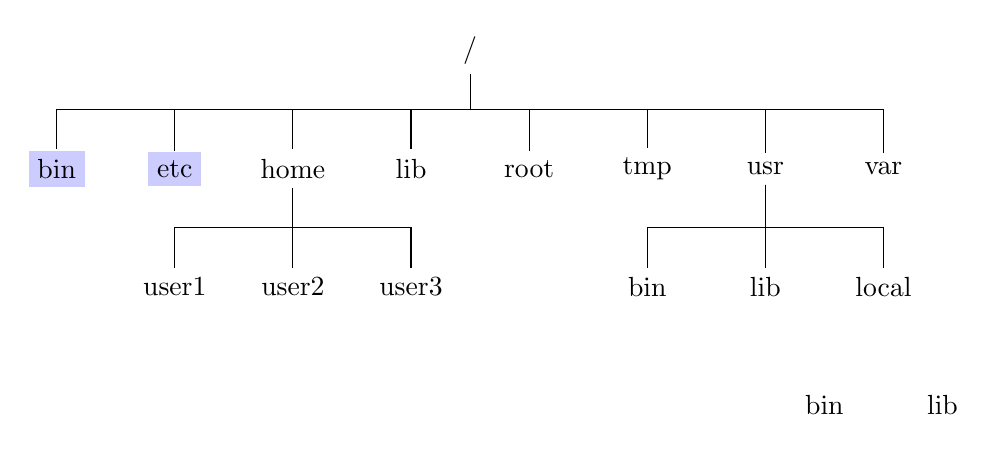
\begin{tikzpicture}
        		        \node{/ }[edge from parent fork down]
                        child{node[rectangle,draw=white, fill=blue!20]{\textcolor{black}{bin}}}
                        child{node[rectangle,draw=white, fill=blue!20]{\textcolor{black}{etc}}}
                        child{node[rectangle,draw=white]{home}
                            child{node[rectangle,draw=white]{user1}}
                            child{node[rectangle,draw=white]{user2}}
                            child{node[rectangle,draw=white]{user3}}}
                        child{node[rectangle,draw=white]{lib}}
                        child{node[rectangle,draw=white]{root}}
                        child{node[rectangle,draw=white]{tmp}}
                        child{node[rectangle,draw=white]{usr}
                            child{node[rectangle,draw=white]{bin}}
                            child{node[rectangle,draw=white]{lib}}
                            child{node[rectangle,draw=white]{local}
                                child[rectangle,draw=white]{node[rectangle,draw=white]{bin}}
                                child[rectangle,draw=white]{node[rectangle,draw=white]{lib}}}}
                        child{node[rectangle,draw=white]{var}}
                        ;
        		    \end{tikzpicture}
        		\end{center}%\vspace{-1cm}
        		\begin{minipage}{0.99\textwidth}
        		    \begin{itemize}
        		        \item[/:] Wurzelverzeichnis
        		        \item[bin:] Systemwichtige Binärdateien
        		        \item[boot:] Dateien zum Starten/Teile des Kernels
        		        \item[dev:] Gerätedateien, Schnittstellen zum Kernel, Kein Speicherbedarf
        		        \item[etc:] Systemweite Einstellungen
        		    \end{itemize}
        		\end{minipage}%
        	\end{frame}
        	
        	\begin{frame}
          		\frametitle{Ordnerhierarchie/backups}
          		\vspace{-1cm}
        		\begin{center}
        		    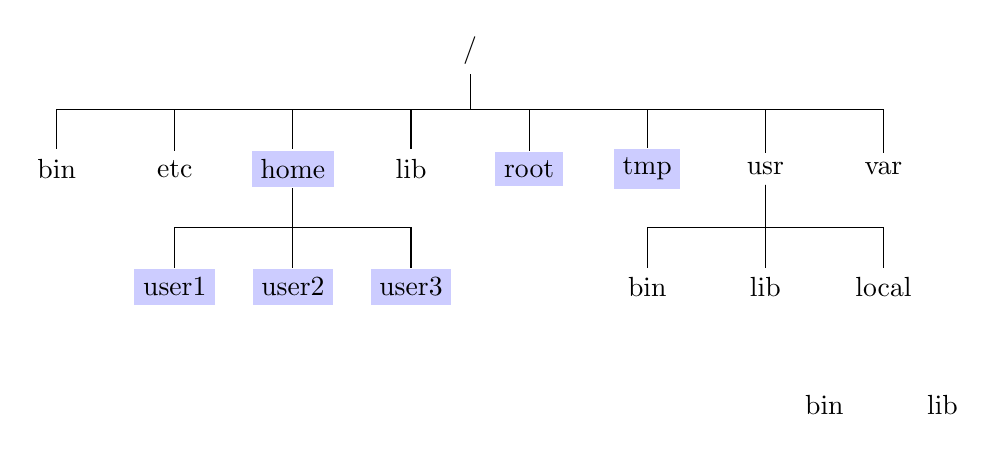
\begin{tikzpicture}
        		        \node{/ }[edge from parent fork down]
                        child{node[rectangle,draw=white]{bin}}
                        child{node[rectangle,draw=white]{etc}}
                        child{node[rectangle,draw=white, fill=blue!20]{\textcolor{black}{home}}
                            child{node[rectangle,draw=white, fill=blue!20]{\textcolor{black}{user1}}}
                            child{node[rectangle,draw=white, fill=blue!20]{\textcolor{black}{user2}}}
                            child{node[rectangle,draw=white, fill=blue!20]{\textcolor{black}{user3}}}}
                        child{node[rectangle,draw=white]{lib}}
                        child{node[rectangle,draw=white, fill=blue!20]{\textcolor{black}{root}}}
                        child{node[rectangle,draw=white, fill=blue!20]{\textcolor{black}{tmp}}}
                        child{node[rectangle,draw=white]{usr}
                            child{node[rectangle,draw=white]{bin}}
                            child{node[rectangle,draw=white]{lib}}
                            child{node[rectangle,draw=white]{local}
                                child[rectangle,draw=white]{node[rectangle,draw=white]{bin}}
                                child[rectangle,draw=white]{node[rectangle,draw=white]{lib}}}}
                        child{node[rectangle,draw=white]{{var}}}
                        ;
        		    \end{tikzpicture}
        		\end{center}
        		\begin{minipage}{0.99\textwidth}
        		    \begin{itemize}
        		        \item[home:] home Verzeichnisse, kann auf anderer Partition liegen.
        		        \item[user$x$:] Verzeichnis von $x$, volle Recht für den Nutzer!
        		        \item[root:] home für den root Nutzer
        		        \item[tmp:] temporäre Dateien, werden bei Start gelöscht 
        		    \end{itemize}
        		\end{minipage}%
        	\end{frame}
        	
        	\begin{frame}
          		\frametitle{Ordnerhierarchie/backups}
          		\vspace{-1cm}
        		\begin{center}
        		    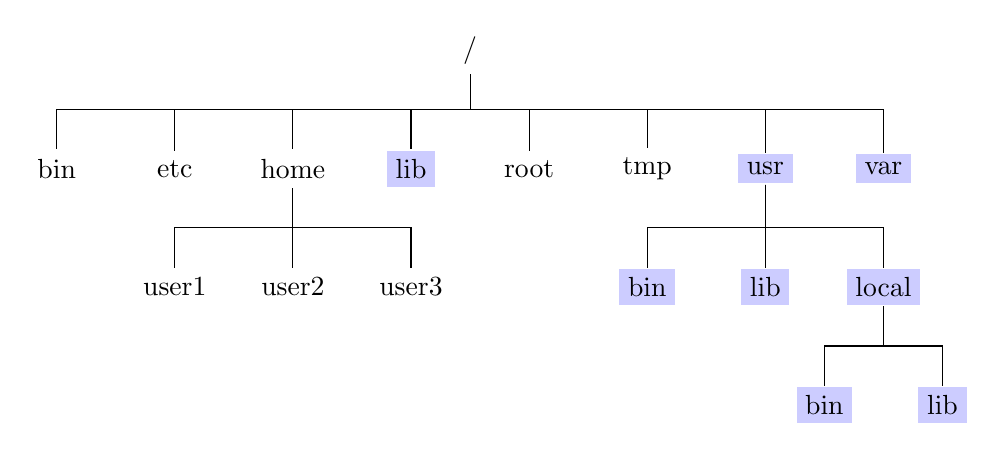
\begin{tikzpicture}
        		        \node{/ }[edge from parent fork down]
                        child{node[rectangle,draw=white]{bin}}
                        child{node[rectangle,draw=white]{etc}}
                        child{node[rectangle,draw=white]{{home}}
                            child{node[rectangle,draw=white]{{user1}}}
                            child{node[rectangle,draw=white]{{user2}}}
                            child{node[rectangle,draw=white]{{user3}}}}
                        child{node[rectangle,draw=white, fill=blue!20]{\textcolor{black}{lib}}}
                        child{node[rectangle,draw=white]{{root}}}
                        child{node[rectangle,draw=white]{{tmp}}}
                        child{node[rectangle,draw=white, fill=blue!20]{\textcolor{black}{usr}}
                            child{node[rectangle,draw=white, fill=blue!20]{\textcolor{black}{bin}}}
                            child{node[rectangle,draw=white, fill=blue!20]{\textcolor{black}{lib}}}
                            child{node[rectangle,draw=white, fill=blue!20]{\textcolor{black}{local}}
                                child {node[rectangle,draw=white, fill=blue!20]{\textcolor{black}{bin}}}
                                child {node[rectangle,draw=white, fill=blue!20]{\textcolor{black}{lib}}}}}
                        child{node[rectangle,draw=white, fill=blue!20]{\textcolor{black}{var}}}
                        ;
        		    \end{tikzpicture}
        		\end{center}
        		\begin{minipage}{0.99\textwidth}
        		    \begin{itemize}
        		        \item[lib:] system bibliotheken.
        		        \item[usr:] \enquote{Unix System Resources}
        		        \item[local:] selbstkompilierte Programme
        		        \item[var:] Häufig neugeschriebene Programmdateien (logs)
        		    \end{itemize}
        		\end{minipage}%
        	\end{frame}
        	
        \subsection{... Nutzer}
            \begin{frame}
          		\frametitle{User/root}
        		\begin{minipage}{0.9\textwidth}
        		    \begin{itemize}
        		        \item Linux ist ein Multiusersystem. (Windows nicht...)
        		        \item Der root user existiert immer, (ID = 0)
        		        \item Beliebig viele User können existieren und parallel arbeiten.
        		    \end{itemize}
        		\end{minipage} 
        		
        		\begin{minipage}{0.54\textwidth}
        		
        		\end{minipage}
        	\end{frame}
        	
        \subsection{... Installation von Software}
            \begin{frame}
          		\frametitle{Installation / Repositories}
        		\begin{minipage}{0.99\textwidth}
        		    \begin{itemize}
        		        \item Software wird \enquote{aus Repositories} installiert.
        		        \item Repositories sind Sammlungen von Software Code, die Entwicklung der Software findet dort statt. 
        		        \item Viele dieser Quellen sind bereits im System vorhanden und können verwendet werden:
        		        \begin{itemize}
        		            \item Softwarecenter (vgl. Android Playstore)
        		            \item via Terminal
        		        \end{itemize}
        		        \item Sollte eine Quelle nicht vorhanden sein, kann sie manuell installiert werden $\to$ Ubuntuwiki
        		    \end{itemize}
        		    Pakete werden also i.R. NICHT bei Chip heruntergeladen ;)
        		\end{minipage}
        	\end{frame}

    \section{Wie verwendet man das dann?}
        \begin{frame}
  		\frametitle{Wie verwendet man das dann?}
    		\begin{center}
        		\begin{minipage}{0.44\textwidth}
        		    \begin{itemize}
        		        \item Beispiel: Thunderbird
        		        \item Beispiel: Installation
        		        \item Beispiel: eduroam?
        		        \item Beispiel: wine
        		    \end{itemize}
        		\end{minipage}%
    		\end{center}
    	\end{frame}
    	
        \subsection{Beispiel: Thunderbird}
            \begin{frame}
          		\frametitle{Einrichtung TB}
        		\begin{minipage}{0.44\textwidth}
        		
        		\end{minipage}%
        		\begin{minipage}{0.54\textwidth}
        		
        		\end{minipage}
        	\end{frame}
        	
        \subsection{Beispiel: Installation Chromium o.Ä.}
            \begin{frame}
          		\frametitle{Installation chromium oder anderer Software}
        		\begin{minipage}{0.44\textwidth}
        		
        		\end{minipage}%
        		\begin{minipage}{0.54\textwidth}
        		
        		\end{minipage}
        	\end{frame}
        
        \subsection{Beispiel: eduroam?}
            \begin{frame}
          		\frametitle{eduroam}
        		\begin{minipage}{0.44\textwidth}
        		
        		\end{minipage}%
        		\begin{minipage}{0.54\textwidth}
        		
        		\end{minipage}
        	\end{frame}
        	
        \subsection{Beispiel: wine}
            \begin{frame}
          		\frametitle{wine -- falls es nicht ohne Windows geht.}
        		\begin{minipage}{0.44\textwidth}
        		
        		\end{minipage}%
        		\begin{minipage}{0.54\textwidth}
        		
        		\end{minipage}
        	\end{frame}
        	
    \section{Hallo! Ich habe eine Problem...}
        \begin{frame}
      		\frametitle{Hallo! Ich habe eine Problem...}
    		\begin{center}
        		\begin{minipage}{0.44\textwidth}
        		    \begin{itemize}
        		        \item Das Ubuntuwiki
        		        \item Terminalbasics
        		    \end{itemize}
        		\end{minipage}%
    		\end{center}
    		\hfill \includegraphics[scale=0.2]{bilder/ohno.png}
    	\end{frame}
    	
        \subsection{Ubuntuwiki}
            \begin{frame}
          		\frametitle{Das Ubuntuwiki}
          		\begin{center}
            		\begin{minipage}{0.44\textwidth}
            		    \url{https://wiki.ubuntu.com/}\vspace{1cm}
            		\end{minipage}\\
            		\begin{minipage}{0.5\textwidth}
            		    \begin{itemize}
            		        \item Begrifflichkeiten
            		        \item Erklärungen
            		        \item Tutorials
            		    \end{itemize} \vspace{1cm}
            		    Google ist dein Freund :)
            		\end{minipage}
        		\end{center}
        	\end{frame}
        	
	    \subsection{Terminalbasics}
    	    \begin{frame}
          		\frametitle{Das Terminal -- BASH}
          		\begin{center}
              		\begin{minipage}{0.60\textwidth}
            		    \begin{itemize}
            		        \item Keine Angst, die Konsole beisst nicht!
            		        \item Öffnen mit Strg + Alt + T
            		    \end{itemize}
            		\end{minipage}%    
          		\end{center}
        		\begin{minipage}{0.50\textwidth}
        		    \begin{itemize}
        		        \item Taskmanager? 
        		        top
        		        \item Abgestürzt? \\
        		        xkill, kill
        		        \item Installation? \\
        		        sudo apt-get (install ...)
        		        \item Dateien zu andeerem Rechner?
        		        scp
        		    \end{itemize}
        		\end{minipage}%
        		\begin{minipage}{0.54\textwidth}
        		    \includegraphics[scale=0.25]{bilder/terminal.png}
        		\end{minipage}
        	\end{frame}
\end{document}
